\documentclass[UTF8]{ctexart}
\usepackage{amsmath,amssymb,graphicx,enumerate,tabularx}

%%%%%%%%%% Start TeXmacs macros
\newcommand{\mathe}{\mathrm{e}}
\newcommand{\tmop}[1]{\ensuremath{\operatorname{#1}}}
\newcommand{\tmrsub}[1]{\ensuremath{_{\textrm{#1}}}}
\newcommand{\tmstrong}[1]{\textbf{#1}}
\newcommand{\tmsubtitle}[1]{\thanks{\textit{Subtitle:} #1}}
\newenvironment{enumerateroman}{\begin{enumerate}[i.] }{\end{enumerate}}
\newenvironment{enumerateromancap}{\begin{enumerate}[I.] }{\end{enumerate}}
%%%%%%%%%% End TeXmacs macros

\begin{document}

\title{
  2022年普通高等学校招生全国统一考试
  \tmsubtitle{数\qquad学}
}

\maketitle

\qquad本试题卷分选择题和非选择题两部分。全卷共4页,选择题部分1至3页;非选择题部分3至4页。满分150分,考试时间120分钟。

\

{\tmstrong{考生注意:}}
\begin{enumerate}
  \item
  答题前,请务必将自己的姓名、准考证号用黑色字迹的签字笔或钢笔分别填写在试题卷和答题纸规定的位置上。
  
  \item
  答题时,请按照答题纸上``注意事项''的要求,在答题纸相应的位置上规范作答,在本试题卷上的作答一律无效。
\end{enumerate}


\begin{multicols}{2}
  {\tmstrong{参考公式:}}
  
  若事件A,B互斥,则
  
  $P (A + B) = P (A) + P (B)$
  
  若事件A,B相互独立,则
  
  $P (\tmop{AB}) = P (A) P (B)$
  
  若事件A在一次试验中发生的概率是$p$,则$n$次独立重复试验中事件$A$恰好发生$k$次的概率
  
  $P_n (k) = C^k_n p^k (1 - p)^{n - k} (k = 0, 1, 2, \ldots, n)$
  
  台体的体积公式
  
  $V = \frac{1}{3} \left( S_1 + \sqrt{S_1 S_2} + S_2 \right) h$
  
  其中$S_1$,
  $S_2$分别表示台体的上、下底面积,$h$表示台体的高
  
  柱体的体积公式
  
  $V = Sh$
  
  其中$S$表示柱体的底面积,h表示柱体的高
  
  锥体的体积公式
  
  $V = \frac{1}{3} Sh$
  
  其中$S$表示锥体的底面积,$h$表示锥体的高
  
  球的表面积公式
  
  $S = 4 \pi R^2$
  
  球的体积公式
  
  $V = \frac{4}{3} \pi R^3$
  
  其中$R$表示球的半径
\end{multicols}

\

\

\begin{center}
  {\tmstrong{选择题部分(共40分)}}
\end{center}

\

{\tmstrong{一、选择题:本大题共10小题,每小题4分,共40分。在每小题给出的四个选项中,只有一项是符合题目要求的。}}
\begin{enumerate}
  \item 设集合$A = \{ 1, 2 \}, B = \{ 2, 4, 6 \}$,则$A \cup B =$
  
  {\noindent}\begin{tabularx}{1.0\textwidth}{@{}X@{}@{}X@{}@{}X@{}@{}X@{}}
    A. $2$ & B. $\{ 1, 2 \}$ & C. $\{ 2, 4, 6 \}$ & D. $\{ 1, 2, 4, 6 \}$
  \end{tabularx}
  
  \item 已知$a, b \in \mathbb{R}, a + 3 i = (b + i)
  i$($i$为虚数单位),则
  
  {\noindent}\begin{tabularx}{1.0\textwidth}{@{}X@{}@{}X@{}@{}X@{}@{}X@{}}
    A. $a = 1, b = - 3$ & B. $a = - 1, b = 3$ & C. $a = - 1, b = - 3$ & D. $a
    = 1, b = 3$
  \end{tabularx}
  
  \item 若实数$x, y$满足约束条件$\left\{\begin{array}{l}
    x - 2 \geqslant 0,\\
    2 x + y - 7 \leqslant 0,\\
    x - y - 2 \leqslant 0,
  \end{array}\right.$则$z = 3 x + 4 y$的最大值是
  
  {\noindent}\begin{tabularx}{1.0\textwidth}{@{}X@{}@{}X@{}@{}X@{}@{}X@{}}
    A. $20$ & B. $18$ & C. $13$ & D. $6$
  \end{tabularx}
  
  \item 设$x \in \mathbb{R}$,则``$\sin x = 1$''是``$\cos x = 0$''的
  
  {\noindent}\begin{tabularx}{1.0\textwidth}{@{}X@{}}
    A. 充分不必要条件\\
    B. 必要不充分条件\\
    C. 充分必要条件\\
    D. 既不充分也不必要条件
  \end{tabularx}
  
  \item
  某几何体的三视图如图所示(单位:cm),则该几何体的体积(单位:$\tmop{cm}^3$)是
  
  {\noindent}\begin{tabularx}{1.0\textwidth}{@{}X@{}@{}X@{}}
    A. $22 \pi$ & B. $8 \pi$\\
    C. $\frac{22}{3} \pi$ & D. $\frac{16}{3} \pi$
  \end{tabularx}
  
  \raisebox{0.0\height}{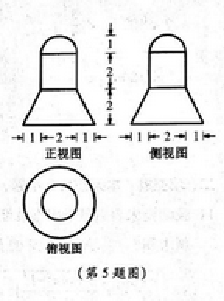
\includegraphics[width=3.7639216843762298cm,height=5.053407451134724cm]{2022年浙江省高考数学试题-1.pdf}}
  
  \item 为了得到函数$y = 2 \sin 3 x$的图象,只要把函数$y = 2
  \sin \left( 3 x + \frac{\pi}{5} \right)$图象上所有的点
  
  {\noindent}\begin{tabularx}{1.0\textwidth}{@{}X@{}@{}X@{}}
    A. 向左平移$\frac{\pi}{5}$个单位长度 & B.
    向右平移$\frac{\pi}{5}$个单位长度\\
    C. 向左平移$\frac{\pi}{15}$个单位长度 & D.
    向右平移$\frac{\pi}{15}$个单位长度
  \end{tabularx}
  
  \item 已知$2^a = 5, \log_8 3 = b$,则$4^{a - 3 b} =$
  
  {\noindent}\begin{tabularx}{1.0\textwidth}{@{}X@{}@{}X@{}}
    A. $25$ & B. $5$\\
    C. $\frac{25}{9}$ & D. $\frac{5}{3}$
  \end{tabularx}
  
  \item 如图,已知正三棱柱$\mathit{ABC} - A_1 B_1 C_1, \mathit{AC} =
  \textit{AA\tmrsub{1}}$,$E, F$分别是棱$\mathit{BC}$,$A_1
  C_1$上的点.记$\mathit{EF}$与$A
  \textit{A\tmrsub{1}}$所成的角为$\alpha$,$\mathit{EF}$与平面$\mathit{ABC}$所成的角为$\beta$,二面角$F
  - \mathit{BC} - A$的平面角为$\gamma$,则
  
  {\noindent}\begin{tabularx}{1.0\textwidth}{@{}X@{}@{}X@{}}
    A. $\alpha \leqslant \beta \leqslant \gamma$ & B. $\beta \leqslant \alpha
    \leqslant \gamma$\\
    C. $\beta \leqslant \gamma < \alpha$ & D. $\alpha \leqslant \gamma <
    \beta$
  \end{tabularx}
  
  {\rendersmallfigure{}{}{\raisebox{-0.30862004106292235\height}{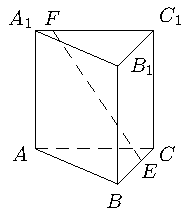
\includegraphics[width=3.1952151383969567cm,height=3.6179489702216974cm]{2022年浙江省高考数学试题-2.pdf}}}{(第8题图)}}
  
  \item 已知$a, b \in \mathbb{R}$,若对任意$x \in \mathbb{R}$,$a | x
  - b | + | x - 4 | - | 2 x - 5 | \geqslant 0$,则
  
  {\noindent}\begin{tabularx}{1.0\textwidth}{@{}X@{}@{}X@{}}
    A. $a \leqslant 1, b \geqslant 3$ & B. $a \leqslant 1, b \leqslant 3$\\
    C. $a \geqslant 1, b \geqslant 3$ & D. $a \geqslant 1, b \leqslant 3$
  \end{tabularx}
  
  \item 已知数列$\{ a_n \}$满足$a_1 = 1, a_{n + 1} = a_n - \frac{1}{3}
  a_n^2 (n \in \mathbb{N}^{\ast})$,则
  
  {\noindent}\begin{tabularx}{1.0\textwidth}{@{}X@{}@{}X@{}}
    A. $2 < 100 a_{100} < \frac{5}{2}$ & B. $\frac{5}{2} < 100 a_{100} < 3$\\
    C. $3 < 100 a_{100} < \frac{7}{2}$ & D. $\frac{7}{2} < 100 a_{100} < 4$
  \end{tabularx}
\end{enumerate}


\

\

\begin{center}
  {\tmstrong{非选择题部分(共110分)}}
\end{center}

\

{\tmstrong{二、填空题:本大题共7小题,单空题每题4分,多空题每空3分,共36分。}}
\begin{enumerate}
  \item
  我国南宋著名数学叫秦九韶,发现了从三角形三边求面积的公式,他把这种方法称为``三斜求积'',它填补了我国传统数学的一个空白.
  如果把这个方法写成公式,就是$S = \sqrt{\frac{1}{4} \left[ c^2
  a^2 - \left( \frac{c^2 + a^2 - b^2}{2} \right)^2 \right]}$,其中$a, b,
  c$是三角形的三边,$S$是三角形的面积.
  设某三角形的三边$a = \sqrt{2}, b = \sqrt{3}, c =
  2$,则该三角形的面积$S =${\underline{{\hspace{3em}}}}.
  
  \item 已知多项式$(x + 2) (x - 1)^4 = a_0 + a_1 x + a_2 x^2 + a_3 x^3 +
  a_4 x^4 + a_5 x^5$,则$a_2 =${\underline{{\hspace{3em}}}}, $a_1 + a_2 +
  a_3 + a_4 + a_5 =${\underline{{\hspace{3em}}}}.
  
  \item 若$3 \sin \alpha - \sin \beta = \sqrt{10}, \alpha + \beta =
  \frac{\pi}{2}$,则$\sin \alpha =${\underline{{\hspace{3em}}}},$\cos 2
  \beta =${\underline{{\hspace{3em}}}}.
  
  \item 已知函数$f (x) = \left\{\begin{array}{ll}
    - x^2 + 2, & x \leqslant 1,\\
    x + \frac{1}{x} - 1, & x > 1,
  \end{array}\right.$则$f \left( f \left( \frac{1}{2} \right) \right)
  =${\underline{{\hspace{3em}}}};若当$x \in [a, b]$时,$1 \leqslant f
  (x) \leqslant 3$,则$b - a$的最大值是{\underline{{\hspace{3em}}}}.
  
  \item 现有 7 张卡片,分别写上数字1,2,3,4,5,6.
  从这7张卡片中随机抽取3张,记所抽取卡片上数字的最小值为$\xi$,则$P
  (\xi = 2) =${\underline{{\hspace{3em}}}},$E (\xi)
  =${\underline{{\hspace{3em}}}}.
  
  \item 已知双曲线$\frac{x^2}{a^2} - \frac{y^2}{b^2} = 1 (a > 0, b >
  0)$的左焦点为$F$,过$F$且斜率为$\frac{b}{4
  a}$的直线交双曲线于点$A (x_1,
  y_1)$,交双曲线的渐近线于点$B (x_2, y_2)$且$x_1 < 0 < x_2$.
  若$| \tmop{FB} | = 3 | \tmop{FA}
  |$,则双曲线的离心率是{\underline{{\hspace{3em}}}}.
  
  \item 设点$P$在单位圆的内接正八边形$A_1 A_2 \ldots
  A_8$的边$A_1 A_2$上,则$\overrightarrow{\tmop{PA}_1}^2 +
  \overrightarrow{\tmop{PA}_2}^2 + \cdots +
  \overrightarrow{\tmop{PA}_8}^2$的取值范围是{\underline{{\hspace{3em}}}}.
\end{enumerate}


\

\

\

\

{\tmstrong{三、解答题:本大题共5小题,共74分。解答应写出文字说明、证明过程或演算步骤。}}
\begin{enumerate}
  \item (本题满分14分)在$\triangle \mathit{ABC}$中,角$A, B,
  C$所对的边分别为$a, b, c$. 已知$4 a = \sqrt{5} c, \cos C =
  \frac{3}{5}$.
  
  (I) 求$\sin A$的值;
  
  (II) 若$b = 11$,求$\triangle \mathit{ABC}$的面积.
  
  \item
  (本题满分15分)如图,已知$\mathit{ABCD}$和$\mathit{CDEF}$都是直角梯形,$\mathit{AB}
  / / \mathit{DC}, \mathit{DC} / / \mathit{EF}, \mathit{AB} = 5, \mathit{DC} =
  3, \mathit{EF} = 1, \angle \mathit{BAD} = \angle \mathit{CDE} =
  60^{\circ}$,二面角$F - \mathit{DC} -
  B$的平面角为$60^{\circ}$,设$M$,$N$分别为$\mathit{AE}$,$\mathit{BC}$的中点.
  
  \begin{multicols}{2}
    (I) 证明:$\mathit{FN} \perp \mathit{AD}$;
    
    (II) 求直线$\mathit{BM}$与平面$\mathit{ADE}$所成角的正弦值.
    
    {\rendersmallfigure{}{}{\raisebox{-0.33117859627858953\height}{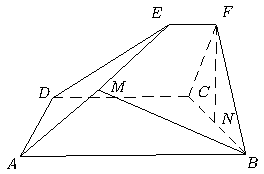
\includegraphics[width=4.437278630460448cm,height=2.922274695001968cm]{2022年浙江省高考数学试题-3.pdf}}}{(第19题图)}}
  \end{multicols}
  
  \item (本题满分15分)已知等差数列$\{ a_n \}$的首项$a_1 = -
  1$,公差$d > 1$. 记$\{ a_n \}$的前$n$项和为$S_n (n \in
  \mathbb{N}^{\ast})$.
  
  (I) 若$S_4 - 2 a_2 a_3 + 6$,求$S_n$;
  
  (II) 若对于每个$n \in \mathbb{N}^{\ast}$,存在实数$c_n$,使$a_n
  + c_n, a_{n + 1} + 4 c_n, a_{n + 2} + 15
  c_n$成等比数列,求$d$的取值范围.
  
  \item (本题满分15分)如图,已知椭圆$\frac{x^2}{12} + y^2 =
  1$. 设$A, B$是椭圆上异与$P (0, 1)$的两点,且点$Q \left( 0,
  \frac{1}{2} \right)$在线段$\mathit{AB}$上,直线$\mathit{PA},
  \mathit{PB}$分别交直线$y = - \frac{1}{2} x + 3$于$C, D$两点.
  
  \begin{multicols}{2}
    (I) 求点$P$到椭圆上点的距离的最大值;
    
    (II) 求$| \mathit{CD} |$的最小值.
    
    \raisebox{0.0\height}{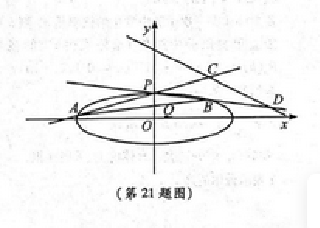
\includegraphics[width=5.367063492063492cm,height=3.8336284927194018cm]{2022年浙江省高考数学试题-4.pdf}}
  \end{multicols}
  
  \item (本题满分15分)设函数$f (x) = \frac{\mathe}{2 x} + \ln x (x
  > 0)$.
  \begin{enumerateromancap}
    \item 求$f (x)$的单调区间;
    
    \item 已知$a, b \in \mathbb{R}$,曲线$y = f
    (x)$上不同的三点$(x_1, f (x_1)), (x_2, f (x_2)), (x_3, f
    (x_3))$处的切线都经过点$(a, b)$. 证明:
    \begin{enumerateroman}
      \item 若$a > \mathe$,则$0 < b - f (a) < \frac{1}{2} \left(
      \frac{a}{e} - 1 \right)$;
      
      \item 若$0 < a < \mathe, x_1 < x_2 < x_3$,则$\frac{2}{\mathe} +
      \frac{\mathe - a}{6 \mathe^2} < \frac{1}{x_1} + \frac{1}{x_3} <
      \frac{2}{a} - \frac{\mathe - a}{6 e^2}$.
    \end{enumerateroman}
  \end{enumerateromancap}
  (注:$e = 2.71828 \ldots$是自然对数的底数)
\end{enumerate}


\end{document}
